\section{Experiments}

\begin{table*}[tbh]
    \centering
    \caption{Quantitative evaluation of the baseline methods and loss functions over different illustration datasets. High values are better and the best one \adding{for the ``Large'' and ``Small'' networks are} presented in bold face.}
    \label{table:quantitative}
    \begin{tabular}{ll cc cc cc cc}
        \toprule
        \multirow{2}{*}{\thead{Group}}     & \multirow{2}{*}{\thead{Method}}           & \multicolumn{2}{c}{\thead{Danbooru2020}} & \multicolumn{2}{c}{\thead{Manga109}} & \multicolumn{2}{c}{\thead{SYNLA (Color)}} & \multicolumn{2}{c}{\thead{SYNLA (Greyscale)}}                                                                       \\
                                           &                                           & \thead{PSNR}                             & \thead{SSIM}                         & \thead{PSNR}                              & \thead{SSIM}                                  & \thead{PSNR}   & \thead{SSIM}    & \thead{PSNR}   & \thead{SSIM}    \\
        \midrule
        \multirow{4}{*}{Competitors}       & Bilinear interpolation                    & 21.42                                    & 0.7806                               & 17.52                                     & 0.6922                                        & 21.19          & 0.7475          & 21.27          & 0.7498          \\
                                           & Bicubic interpolation                     & 21.97                                    & 0.8026                               & 18.01                                     & 0.7190                                        & 22.29          & 0.7977          & 22.37          & 0.7996          \\
                                           & Baseline                                  & 23.08                                    & 0.8274                               & 19.31                                     & 0.7726                                        & 22.50          & 0.7638          & 24.23          & 0.8493          \\
                                           & Baseline-RGB                              & 22.47                                    & 0.7878                               & 18.73                                     & 0.7328                                        & 22.39          & 0.7660          & 23.73          & 0.8410          \\
        \midrule
        \multirow{6}{*}{Large CNN (Ours)}  & Mean Absolute Error                       & \textbf{26.86}                           & 0.9351                               & \textbf{21.43}                            & 0.8559                                        & \textbf{25.60} & \textbf{0.8928} & \textbf{27.17} & \textbf{0.9301} \\
                                           & Mean Squared Error                        & 26.58                                    & 0.9233                               & 19.88                                     & 0.8027                                        & 23.28          & 0.7882          & 24.68          & 0.8783          \\
                                           & Mixed Gradient Error ($\lambda_G = 1.00$) & 26.60                                    & 0.9220                               & 21.18                                     & 0.8443                                        & 25.04          & 0.8564          & 26.24          & 0.9055          \\
                                           & Multi-scale Structural Dissimilarity      & 25.47                                    & 0.9069                               & 20.76                                     & 0.8270                                        & 23.99          & 0.8198          & 25.03          & 0.8817          \\
                                           & Perceptual Loss without Pooling           & 26.39                                    & 0.9022                               & 20.93                                     & 0.8269                                        & 23.86          & 0.7902          & 25.80          & 0.8831          \\
                                           & Structural Dissimilarity                  & 26.62                                    & \textbf{0.9369}                      & 21.17                                     & \textbf{0.8584}                               & 25.23          & 0.8889          & 26.60          & 0.9300          \\
        \midrule
        \multirow{10}{*}{Small CNN (Ours)} & Mean Absolute Error                       & 23.14                                    & 0.8402                               & 19.07                                     & 0.7751                                        & 22.58          & 0.7831          & 24.34          & 0.8655          \\
                                           & Mean Squared Error                        & 23.99                                    & 0.8514                               & 20.12                                     & 0.8040                                        & 23.14          & 0.7816          & 24.84          & 0.8663          \\
                                           & Mixed Gradient Loss ($\lambda_G = 0.01$)  & 24.61                                    & \textbf{0.8708}                      & 20.62                                     & \textbf{0.8235}                               & 23.30          & 0.7864          & \textbf{25.35} & 0.8791          \\
                                           & Mixed Gradient Loss ($\lambda_G = 0.10$)  & 24.62                                    & 0.8700                               & \textbf{20.65}                            & 0.8216                                        & 23.22          & 0.7858          & 25.31          & 0.8776          \\
                                           & Mixed Gradient Loss ($\lambda_G = 1.00$)  & 24.66                                    & 0.8707                               & 20.63                                     & 0.8231                                        & 23.24          & 0.7839          & 25.17          & 0.8746          \\
                                           & Multi-scale Structural Dissimilarity      & 24.04                                    & 0.8684                               & 20.01                                     & 0.8111                                        & \textbf{23.47} & \textbf{0.8139} & 24.85          & \textbf{0.8815} \\
                                           & Pencil Sketch                             & 24.00                                    & 0.8393                               & 20.24                                     & 0.7817                                        & 21.90          & 0.7159          & 24.35          & 0.8439          \\
                                           & Perceptual Loss without Pooling           & \textbf{24.73}                           & 0.8566                               & 20.64                                     & 0.8176                                        & 23.08          & 0.7636          & 25.30          & 0.8700          \\
                                           & Perceptual Loss with Pooling              & 22.55                                    & 0.7298                               & 19.07                                     & 0.7368                                        & 20.81          & 0.6347          & 21.33          & 0.7105          \\
                                           & Structural Dissimilarity                  & 23.12                                    & 0.8600                               & 19.34                                     & 0.7949                                        & 22.37          & 0.8013          & 23.93          & 0.8751          \\
        \bottomrule
    \end{tabular}
\end{table*}

In this section, we provide details about the implementation, datasets, experimental evaluation, and its results.

\subsection{Small network configuration}

To perform the experiments, we implement the modified version of the ESPCN CNN presented in Section~\ref{section:methodology/architectures} and illustrated in Figure~\ref{figure:espcn}. The architecture is composed of {$64$ $5\times 5$} feature maps in the first layer, {$32$ $3\times 3$} in the second, and $27$ $3\times 3$ in the last, totaling $31\,131$ learnable parameters.

For each evaluated loss function, this network was trained for up to $1500$ epochs; the training process was halted after no improvements in the loss function were shown on the validation dataset for $100$ epochs. The learning rate was set to ${\alpha = 10^{-3}}$ on the first two convolution layers of the network and $10^{-4}$ on the last, with no scheduling, as reported by the authors~\cite{shi2016realtime}.

We trained three networks in order to observe the effects of the $\lambda_{G}$ hyperparameter in the MixGE loss function.

\subsection{\adding{Large network configuration}}

In order to confirm whether our hypothesis that a loss function will perform the same across network depths, we evaluated a residual network outlined in Section~\ref{section:methodology/architectures} and Figure~\ref{figure:residual} with $4\,756\,388$ parameters, referred to as our \textbf{Large} network.

Due to hardware availability constraints, only the following subset of the loss functions were evaluated in this network:
\begin{enumerate*}
    \item Mean Absolute Error;
    \item Mean Squared Error;
    \item Mixed Gradient Error with $\lambda_G = 1.00$;
    \item Multi-scale Structural Dissimilarity;
    \item Perceptual Loss without Max Pooling;
    \item Structural Dissimilarity.
\end{enumerate*}

For each loss function, this network was trained for up to $1500$ epochs; the training process was halted after no improvements in the loss function were shown on the validation dataset for $50$ epochs. The initial learning rate was set to ${\alpha = 10^{-3}}$ and was multiplied by $0.1$ on every 50th epoch.

\subsection{Input and Output data}

Our experiments were executed on RGB images set to be upscaled by a factor of $3$. We used the central patch of each image as the high-resolution target, and prepared the low-resolution inputs by blurring the target with a Gaussian kernel of ${\sigma = 1.0}$ before downsampling with bicubic interpolation by a factor of $3$.

\adding{In both network architectures, each color channel of the input images were approximated into a standard normal distribution through the following normalization step:}

\begin{equation}
    \hat{x}_{\text{Channel}} = \frac{x_{\text{Channel}} - \mu_{\text{Channel}}}{\sigma_{\text{Channel}}} \text{,}
\end{equation}

\noindent where $\mu_{\text{Red}} = 0.7026$, $\sigma_{\text{Red}} = 0.2931$, $\mu_{\text{Green}} = 0.6407$, $\sigma_{\text{Green}} = 0.2985$, $\mu_{\text{Blue}} = 0.6265$ and $\sigma_{\text{Blue}} = 0.2946$, obtained by calculating the mean and standard deviation of the training dataset.

In the large network, this transformation was then reversed at the network output through the following formula:

\begin{equation}
    \hat{y}_{\text{Channel}} = y_{\text{Channel}} \cdot \sigma_{\text{Channel}} + \mu_{\text{Channel}} \text{.}
\end{equation}

\subsection{\adding{Perceptual Loss}}

The first components of a neural network pre-trained by a third-party\footnote{Available at:~https://rf5.github.io/2019/07/08/danbuuro-pretrained.html} were used as the feature extractor $\phi$ for the perceptual loss.
Two experiments were conducted with this loss, in which said components were:
\begin{enumerate*}
    \item a $7\times7$ convolution layer with stride 2 and 64 filters, followed by a batch normalization layer and the ReLU activation function;
    \item the same as previous item, except for the addition of a max pooling layer.
\end{enumerate*}
Both versions of the $\phi$ feature extractor had $9\,536$ parameters.


% The original network was trained to solve a multi-class classification problem on illustrations and is publicly available : Essa parte eu não entendi. É um rede de 1 camada  convolucional com 64 filtros? E depois? Tem uma FC? Como isso foi treinado para esse problema?}\footnote{Project page:~https://rf5.github.io/2019/07/08/danbuuro-pretrained.html}.

% A \review{shallow : o que é esse Shallow subset?} subset with $9\,536$ parameters from a classifier network was used as the feature extractor $\phi$ for the perceptual loss, containing 64 $7 \times 7$ convolutions with stride 2. 



\subsection{Datasets}
\label{section:datasets}


In an attempt to replicate the wide spectrum of illustrations, the following three datasets were used in this work.

\subsubsection{Danbooru2020}

A collection of approximately $4$ million crowdsourced illustrations~\cite{danbooru2020}\footnote{Publicly available at \url{https://www.gwern.net/Danbooru2020}.} of varying characteristics, ranging from line art to highly textured pictures. A subset of $40$ thousand randomly sampled images were selected for use during the training phase, of which $8$ thousand were used for validation at the end of each epoch. A second subset of $10$ thousand images was used for testing. Due to hardware constraints for training, we used ${96\times96}$ central patches as the ground truth images.

\subsubsection{Manga109}
\label{subsection:manga109}

A collection of approximately 10 thousand comic pages drawn by professional manga artists in Japan~\cite{mtap_matsui_2017,multimedia_aizawa_2020}\footnote{Available upon request at \url{http://www.manga109.org/en/}.} used as a benchmark for SISR tasks \cite{haris2018deep,zhang2018residual}. This dataset is characterized by having mostly grayscale images with finer details such as text. We used ${288\times288}$ central patches from this dataset as the ground truth images. A larger patch size was used in order to capture a meaningful section of the illustration images present in this dataset.

\subsubsection{SYNLA}

In order to further evaluate the generalization capabilities of the networks and find potential pathological cases, we also included a collection of synthetic line art images~\cite{synla}\footnote{Publicly available at \url{https://github.com/bloc97/SYNLA-Dataset}.}. The dataset is available in two versions, each with roughly $2000$ images, both which were used: one in grayscale, the other in color. As the original image sizes were smaller than the patch size ${288\times288}$, specified in Section~\ref{subsection:manga109}, and not an exact multiple of our scale factor, we used ${192\times192}$ central patches from this dataset as the ground truth images.

Danbooru2020 was used for training and testing, due to its wide range of illustrations in order to train networks able to generalize over style characteristics. Manga109 and SYNLA were used solely for testing.

\subsection{Competitors}

We compare our proposed models with the following approaches:

\begin{description}
    \item[Baseline]
          A pre-trained\footnote{Publicly available in: \url{https://github.com/Lornatang/ESPCN-PyTorch}} ESPCN~\cite{shi2016realtime} model, using as input the Y-channel of the image in YCbCr color space.
          This network was trained with the DIV2K~\cite{Agustsson_2017_CVPR_Workshops} dataset and the MSE loss function.

    \item[Baseline-RGB]
          The ESPCN model with RGB images as input, trained in the DIV2k dataset, MSE loss function, using the same network configuration and training parameters of our methods.

    \item[Bilinear and Bicubic]
          These interpolations methods were also included in order to establish a lower bound for effectiveness: \adding{a deep learning model that performs worse than either of them may be undesirable, as both interpolation methods are well-understood and computationally cheap.}
\end{description}

\section{Results}

\begin{figure*}[tbhp]
    \centering

    \subfloat[Input]{
        \includegraphics[width=0.135\linewidth]{figs/SR/LR}
    }
    \subfloat[Ground Truth]{
        \includegraphics[width=0.135\linewidth]{figs/SR/HR}
    }
    \subfloat[Bicubic]{
        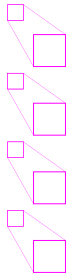
\includegraphics[width=0.135\linewidth]{figs/SR/Bicubic}
    }
    \subfloat[Baseline]{
        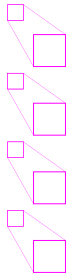
\includegraphics[width=0.135\linewidth]{figs/SR/Photography}
        \label{figure:comparisons/baseline}
    }
    \subfloat[Ours (MAE)]{
        \includegraphics[width=0.135\linewidth]{figs/SR/Ours@ESPCN@L1}
        \label{figure:comparisons/mae}
    }
    \subfloat[Ours (MSE)]{
        \includegraphics[width=0.135\linewidth]{figs/SR/Ours@ESPCN@L2}
        \label{figure:comparisons/mse}
    }
    \smallbreak
    \subfloat[Ours (DSSIM)]{
        \includegraphics[width=0.135\linewidth]{figs/SR/Ours@ESPCN@SSIM}
        \label{figure:comparisons/dssim}
    }
    \subfloat[Ours (MS-DSSIM)]{
        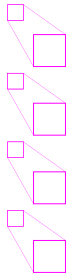
\includegraphics[width=0.135\linewidth]{figs/SR/Ours@ESPCN@MS-SSIM}
        \label{figure:comparisons/ms-dssim}
    }
    \subfloat[Ours (MixGE)]{
        \includegraphics[width=0.135\linewidth]{figs/SR/Ours@ESPCN@Sobel001}
        \label{figure:comparisons/mixge}
    }
    \subfloat[Ours (Sketch)]{
        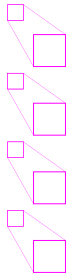
\includegraphics[width=0.135\linewidth]{figs/SR/Ours@ESPCN@Sketch}
        \label{figure:comparisons/sketch}
    }
    \subfloat[Ours (Perceptual)]{
        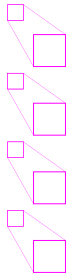
\includegraphics[width=0.135\linewidth]{figs/SR/Ours@ESPCN@Perceptual}
        \label{figure:comparisons/perceptual}
    }

    \caption[]{
        Comparison across loss functions on the \textbf{Small} network.
        Regions outlined in magenta are magnified to better visualize the impact of applying different SISR methods. ``Ours (MixGE)'' uses $\lambda_G = 0.01$ and the Baseline is the pre-trained Y-channel ESPCN model.
        From top to bottom rows, images are cropped samples of the following sources:
        \begin{enumerate*}
            \item Manga109\cite{mtap_matsui_2017,multimedia_aizawa_2020}, \copyright~Ken~Akamatsu\label{figure:manga109}
            \item Wikipedia (\url{https://en.wikipedia.org/wiki/File:Wikipe-tan_face.svg})
            \item SYNLA dataset\cite{synla}
            \item Set14 dataset\cite{zeyde2010single}.
        \end{enumerate*}
    }

    \label{figure:comparisons}
\end{figure*}



\begin{figure*}[h!]
    \centering

    \subfloat[Input]{
        \includegraphics[width=0.11\linewidth]{figs/SR/LR}
    }
    \subfloat[Ground Truth]{
        \includegraphics[width=0.11\linewidth]{figs/SR/HR}
    }
    \subfloat[MAE]{
        \includegraphics[width=0.11\linewidth]{figs/SR/Ours@Residual@L1}
    }
    \subfloat[MSE]{
        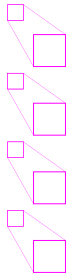
\includegraphics[width=0.11\linewidth]{figs/SR/Ours@Residual@L2}
        \label{figure:comparisons/large/mse}
    }
    \subfloat[SSIM]{
        \includegraphics[width=0.11\linewidth]{figs/SR/Ours@Residual@SSIM}
    }
    \subfloat[MS-SSIM]{
        \includegraphics[width=0.11\linewidth]{figs/SR/Ours@Residual@MS-SSIM}
    }
    \subfloat[Perceptual]{
        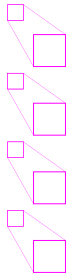
\includegraphics[width=0.11\linewidth]{figs/SR/Ours@Residual@Perceptual}
    }
    \subfloat[MixGE]{
        \includegraphics[width=0.11\linewidth]{figs/SR/Ours@Residual@Sobel}
    }
    \caption{
        Comparison across loss functions on our \textbf{Large} network. See Figure~\ref{figure:comparisons} for image sources.
    }

    \label{figure:comparisons-large}
\end{figure*}


In this section, we discuss the results obtained from training the neural networks with the loss functions discussed through the work, presented in Table~\ref{table:quantitative}. We also present a few handpicked samples in Figure~\ref{figure:comparisons} and Figure~\ref{figure:comparisons-large} for discussion as part of our qualitative analysis. 

Two images which did not originate from the datasets listed in Section~\ref{section:datasets} were included for qualitative analysis: the image in the fourth row is an illustration frequently used as a test case across super-resolution works. The level of details in this image reduces the gap between the result obtained from the baseline network (Figure~\ref{figure:comparisons/baseline}) and our best result (Figure~\ref{figure:comparisons/mixge}). \adding{The image in the second row was included as a sample vectorial illustration image, allowing the generation of a low-resolution input without downsampling artifacts.}

\subsection{Analysis on the small network}

From experimental observations, the $\MAE$ caused the training process to reach a plateau after the least number of iterations among the studied functions, followed by the Pencil Sketch, $\DSSIM$. The training process persisted for the $\MSE$, the $\MSDSSIM$, the perceptual loss and the mixed gradient error until the upper limit of 1500 epochs.

While the images produced by the network trained with the MAE loss have less noise than the one trained with the MSE, it has caused aliased edges in flat images, such as the second row in Figure~\ref{figure:comparisons/mae}, motivating further exploration.

It was observed that the DSSIM led the network to optimize for edge restoration at the expense of accuracy in color reproduction.
In the second row of Figure~\ref{figure:comparisons/dssim}, the image has less noise than its counterparts, but the colorization of the character is visibly different.
This can also be observed in the first row: the image has a slight red hue compared to its grayscale counterparts.
While this did not occur in the network trained with the $\MSDSSIM$ loss (Figure~\ref{figure:comparisons/ms-dssim}), the images produced by it are also noisier.

\begin{figure}[htbp]
    \centering

    \subfloat[MixGE]{
        \includegraphics[width=0.45\linewidth]{figs/SR/Wikipe-tan/Ours@ESPCN@Sobel001}
        \label{fig:comparison/wiki-ours}
    }
    \subfloat[Baseline]{
        \includegraphics[width=0.45\linewidth]{figs/SR/Wikipe-tan/Photography}
        \label{fig:comparison/wiki-photo}
    }
    \smallbreak
    \subfloat[MixGE]{
        \includegraphics[width=0.45\linewidth]{figs/SR/SYNLA@Color/Ours@ESPCN@Sobel001}
        \label{fig:comparison/synla-ours}
    }
    \subfloat[Baseline]{
        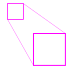
\includegraphics[width=0.45\linewidth]{figs/SR/SYNLA@Color/Photography}
        \label{fig:comparison/synla-photo}
    }

    \caption{
        \label{fig:comparison}
        Comparison of the photography-centric baseline against the small network trained with the MixGE loss ($\lambda_G = 0.01$).
        Figure~\ref{fig:comparison/wiki-ours} depicts a case where the neural network trained on the gradient loss produces smoother edges.
        Figure~\ref{fig:comparison/synla-ours} depicts a pathological case with excessive production of noise.
    }
\end{figure}

As seen in Table~\ref{table:quantitative}, variations of the MixGE loss function have led to the best results in most recorded metrics. While it has been observed to reconstruct well in general scenarios, images restored from blurry low-resolution pictures, such as the image in the second row in Figure~\ref{figure:comparisons}, have shown the highest incidence of noise among the trained networks, as seen in Figure~\ref{fig:comparison}, characterizing a pathological case.

Our experiments showed little to no impact in assigning three different weights ($0.01$, $0.10$, $1.00$) to the $\lambda_G$ gradient component of the MixGE loss --- as seen in Table~\ref{table:quantitative}, metric results were close to each other and no discernible differences were observed in an analysis of the reconstructed images.

Despite their similar formulation, the Pencil Sketch loss function (Figure~\ref{figure:comparisons/sketch}) did not show comparable performance to the Mixed Gradient Error, having substantially lower scores across the board and producing noisier images.
We also found this loss function to be inherently unstable during the training, sometimes causing divisions by zero despite the stabilizing term. This instability may be attributed to the network output being unconstrained: during the early stages of training, a randomly initialized network can produce values which causes a division by zero in Equation~\ref{equation:sketch}, despite the stabilizing term $\epsilon$, making this loss function unsuitable for such cases.

The Perceptual Loss (Figure~\ref{figure:comparisons/perceptual}) has shown similar quality characteristics as the Mixed Gradient Error: in images with solid regions, it produces less noise than the alternatives while producing more of such artifacts in blurry images.

We also observed that the depth of the chosen feature descriptor $\phi$ entails a trade-off: a shallow descriptor may optimize only for lower-level features, such as drawing primitives, while a deep descriptor may discard details deemed unnecessary to the task for which it was previously trained, potentially causing undesirable artifacts, as seen in Figure~\ref{figure:perceptual/comparison}. 
This was explored through the inclusion and omission of a pooling layer in the feature descriptor: because the noise information is discarded by the feature extractor with the pooling, it is not back-propagated, causing the reconstructed image in Figure~\ref{figure:perceptual/with-maxpool} to be unconstrained and have artifacts that would otherwise not be present, as in Figure~\ref{figure:perceptual/without-maxpool}.

\begin{figure}[htbp]
    \centering
    \label{figure:perceptual/comparison}

    \subfloat[\label{figure:perceptual/without-maxpool}Without Max Pooling]{
        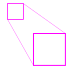
\includegraphics[width=0.45\linewidth]{figs/perceptual/BeforeMaxPool}
    }
    \subfloat[\label{figure:perceptual/with-maxpool}With Max Pooling]{
        \includegraphics[width=0.45\linewidth]{figs/perceptual/AfterMaxPool}
    }
    \caption{
        Effects of the inclusion and omission of a pooling operation in a feature descriptor.
    }
\end{figure}

Regarding the modifications applied to the ESPCN architecture, we observe that the addition of the non-parametric normalization layer at the start of the network helped the training process by making the model to learn faster.

\subsection{\label{section:analysis-large-network}Analysis on the large network}

In regards to the larger network, three factors that particularly stand out in Table~\ref{table:quantitative} and in Figure~\ref{figure:comparisons-large} are described in this section.

The Mean Squared Error network yielded substantially worse results than all of the other large networks, producing a large amount of noise artifacts in the images, shown in Figure~\ref{figure:comparisons/large/mse}. This has caused the network to produce results with worse visual quality than the ones produced by the small network (Figure~\ref{figure:comparisons}), despite higher metric scores.

Contrary to our previous expectations that a loss function would retain its performance characteristics across network size, Table~\ref{table:quantitative} shows that this may not be true in practice: the Structural Dissimilarity and the Mean Absolute Error, which performed poorly on the smaller network, yielded the best metric results.

With exception of the Mean Squared Error and the Multi-scale Structural Similarity networks, most results are visually indistinguishable. This could be explained by considering that a sufficiently large network may be able to learn all of the characteristics of a training dataset, rendering the intrinsic prioritization of a loss function redundant.
